\documentclass{beamer}
\setbeamertemplate{navigation symbols}{} % eliminate navigation bar
\usetheme{CambridgeUS}

\usefonttheme{structurebold}
% Arch Linux Color Theme
\definecolor{arch}{RGB}{23,147,209}
\usecolortheme[named=arch]{structure}
\usecolortheme{whale}
\setbeamercolor{frametitle}{bg=arch!80!black}
\setbeamercolor{title}{bg=arch!90!black}

\usepackage{lmodern}
\usepackage[utf8]{inputenc}
\usepackage[american]{babel}

\usepackage{graphicx}

\usepackage{listings}
\lstset{
  basicstyle=\ttfamily\footnotesize,
  stringstyle=\color{Plum}\slshape,
  commentstyle=\color{OliveGreen},
  keywordstyle=\color{Plum},
  showstringspaces=false,
  tabsize=2,
  frame=single,
  basicstyle=\tiny
}


%\usepackage{listings}
%\lstset{language=Java,
%  basicstyle=\ttfamily\small,
%  tabsize=2}

\newcommand{\backupbegin}{
  \newcounter{finalframe}
  \setcounter{finalframe}{\value{framenumber}}
}
\newcommand{\backupend}{
  \setcounter{framenumber}{\value{finalframe}}
}

\setbeamercovered{transparent=20}


%% META INFORMATION ABOUT DOCUMENT
% \title[short]{long}
% short argument is used in places where there is little space
% long is used on the title slide

\title[Refactoring]{Refactoring Techniques and Automated Approaches Through Tool Support}
\subtitle{Seminar in Software Engineering}
\institute[]{Institute for Software Systems Engineering\\Johannes Kepler University Linz}

\subject{Automated Refactoring}

\pgfdeclareimage[height=0.5cm]{isse-logo}{bilder/isse}
\logo{\pgfuseimage{isse-logo}}

\author[Feichtinger, Kritzinger]{Peter Feichtinger\texorpdfstring{\\}{, }Lisa Kritzinger} % Variante: \and

\date{13. June 2017}


\begin{document}

%% TITLE PAGE
\begin{frame}
  \titlepage
\end{frame}

% for longer presentations table of contents is useful
\begin{frame}
  \frametitle{Outline}
  \tableofcontents[] 
\end{frame}


\section{Introduction}  % always defined outside a frame, optional short argument

\begin{frame}{Refactoring}
  \begin{itemize}
    \item Restructuring code without change in semantics
    \begin{itemize}
      \item Importance in software evolution is obvious
      \item Tool support is important
    \end{itemize}
  \end{itemize}
  \pause
  \begin{itemize}
    \item Topics:
    \begin{itemize}
      \item Performance impact of refactoring
      \item Modernizing code
      \item Automated refactoring
    \end{itemize}
  \end{itemize}
\end{frame}

\subsection{Automated Refactoring in General}

\begin{frame}{Automated Refactoring}
  \begin{itemize}
    \item Goals
    \begin{itemize}
      \item Understandability
      \item Correctness
      \item Ease of Maintenance and Evolution
    \end{itemize}
  \end{itemize}
  \pause
  \begin{itemize}
    \item Automated Refactoring Steps
    
      \visible<2>{\vspace{4pt}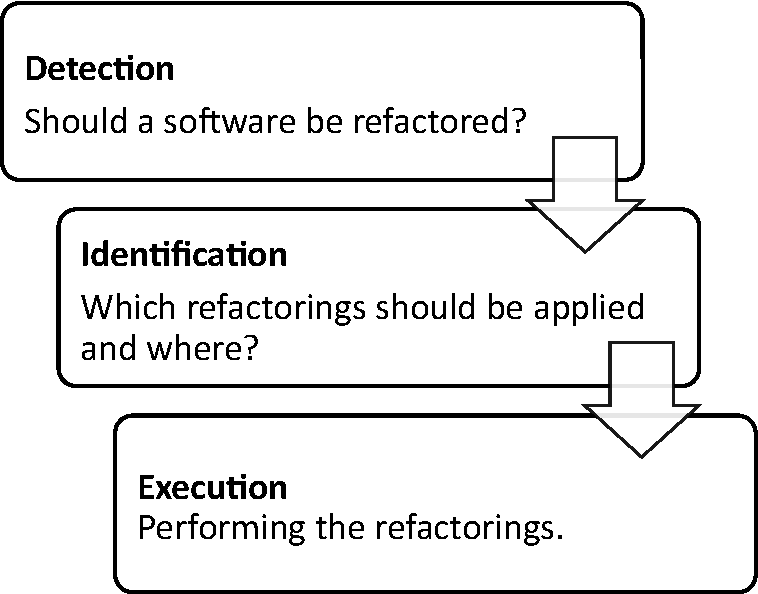
\includegraphics[width=0.4\linewidth]{bilder/process}}
  \end{itemize}
\end{frame}

\section{Automated Refactoring Approaches}

\subsection{Restructuring Legacy C Code into C++}

\begin{frame}{Restructuring Legacy C Code into C++}
  
  \begin{itemize}
    \item Case study on Mosaic browser code
    \pause
    \item Combination of refactorings to create classes
    \begin{itemize}
      \item From C \texttt{struct}s
      \item From related variables
    \end{itemize}
  \end{itemize}
\end{frame}

\subsection{Performance Impact of Polymorphism}

\begin{frame}{Performance Impact of Polymorphism}
  
  \begin{itemize}
    \item Comparison of the performance of two programms
    \begin{itemize}
      \item one which contains large conditionals
      \item one where the conditionals are implemented using polymorphism
    \end{itemize}
  \end{itemize}
\end{frame}

\begin{frame}[fragile]{Performance Impact of Polymorphis}
  \begin{columns}[T]
    \begin{column}{.49\textwidth}
      \lstinputlisting{code/ConditionalWidget.cpp}
    \end{column}
    \begin{column}{.5\textwidth}
      \lstinputlisting{code/PolymorphicWidget.cpp}
    \end{column}
  \end{columns}
\end{frame}

\subsection{Design Differencing}

\begin{frame}{Design Differencing}
  
  \begin{itemize}
    \item Novel refactoring approach that refactors a program based on 
    \begin{itemize}
      \item desired design
      \item source code
    \end{itemize}
    \pause
    \item Using desired design as target, based on
    \begin{itemize}
      \item current software design and
      \item understanding of how it may be required to evolve
    \end{itemize}
  \end{itemize}
\end{frame}

\begin{frame}{Design Differencing}
  \begin{columns}[T]
    \begin{column}{.5\textwidth}
      \begin{figure}[t]
        \centering
        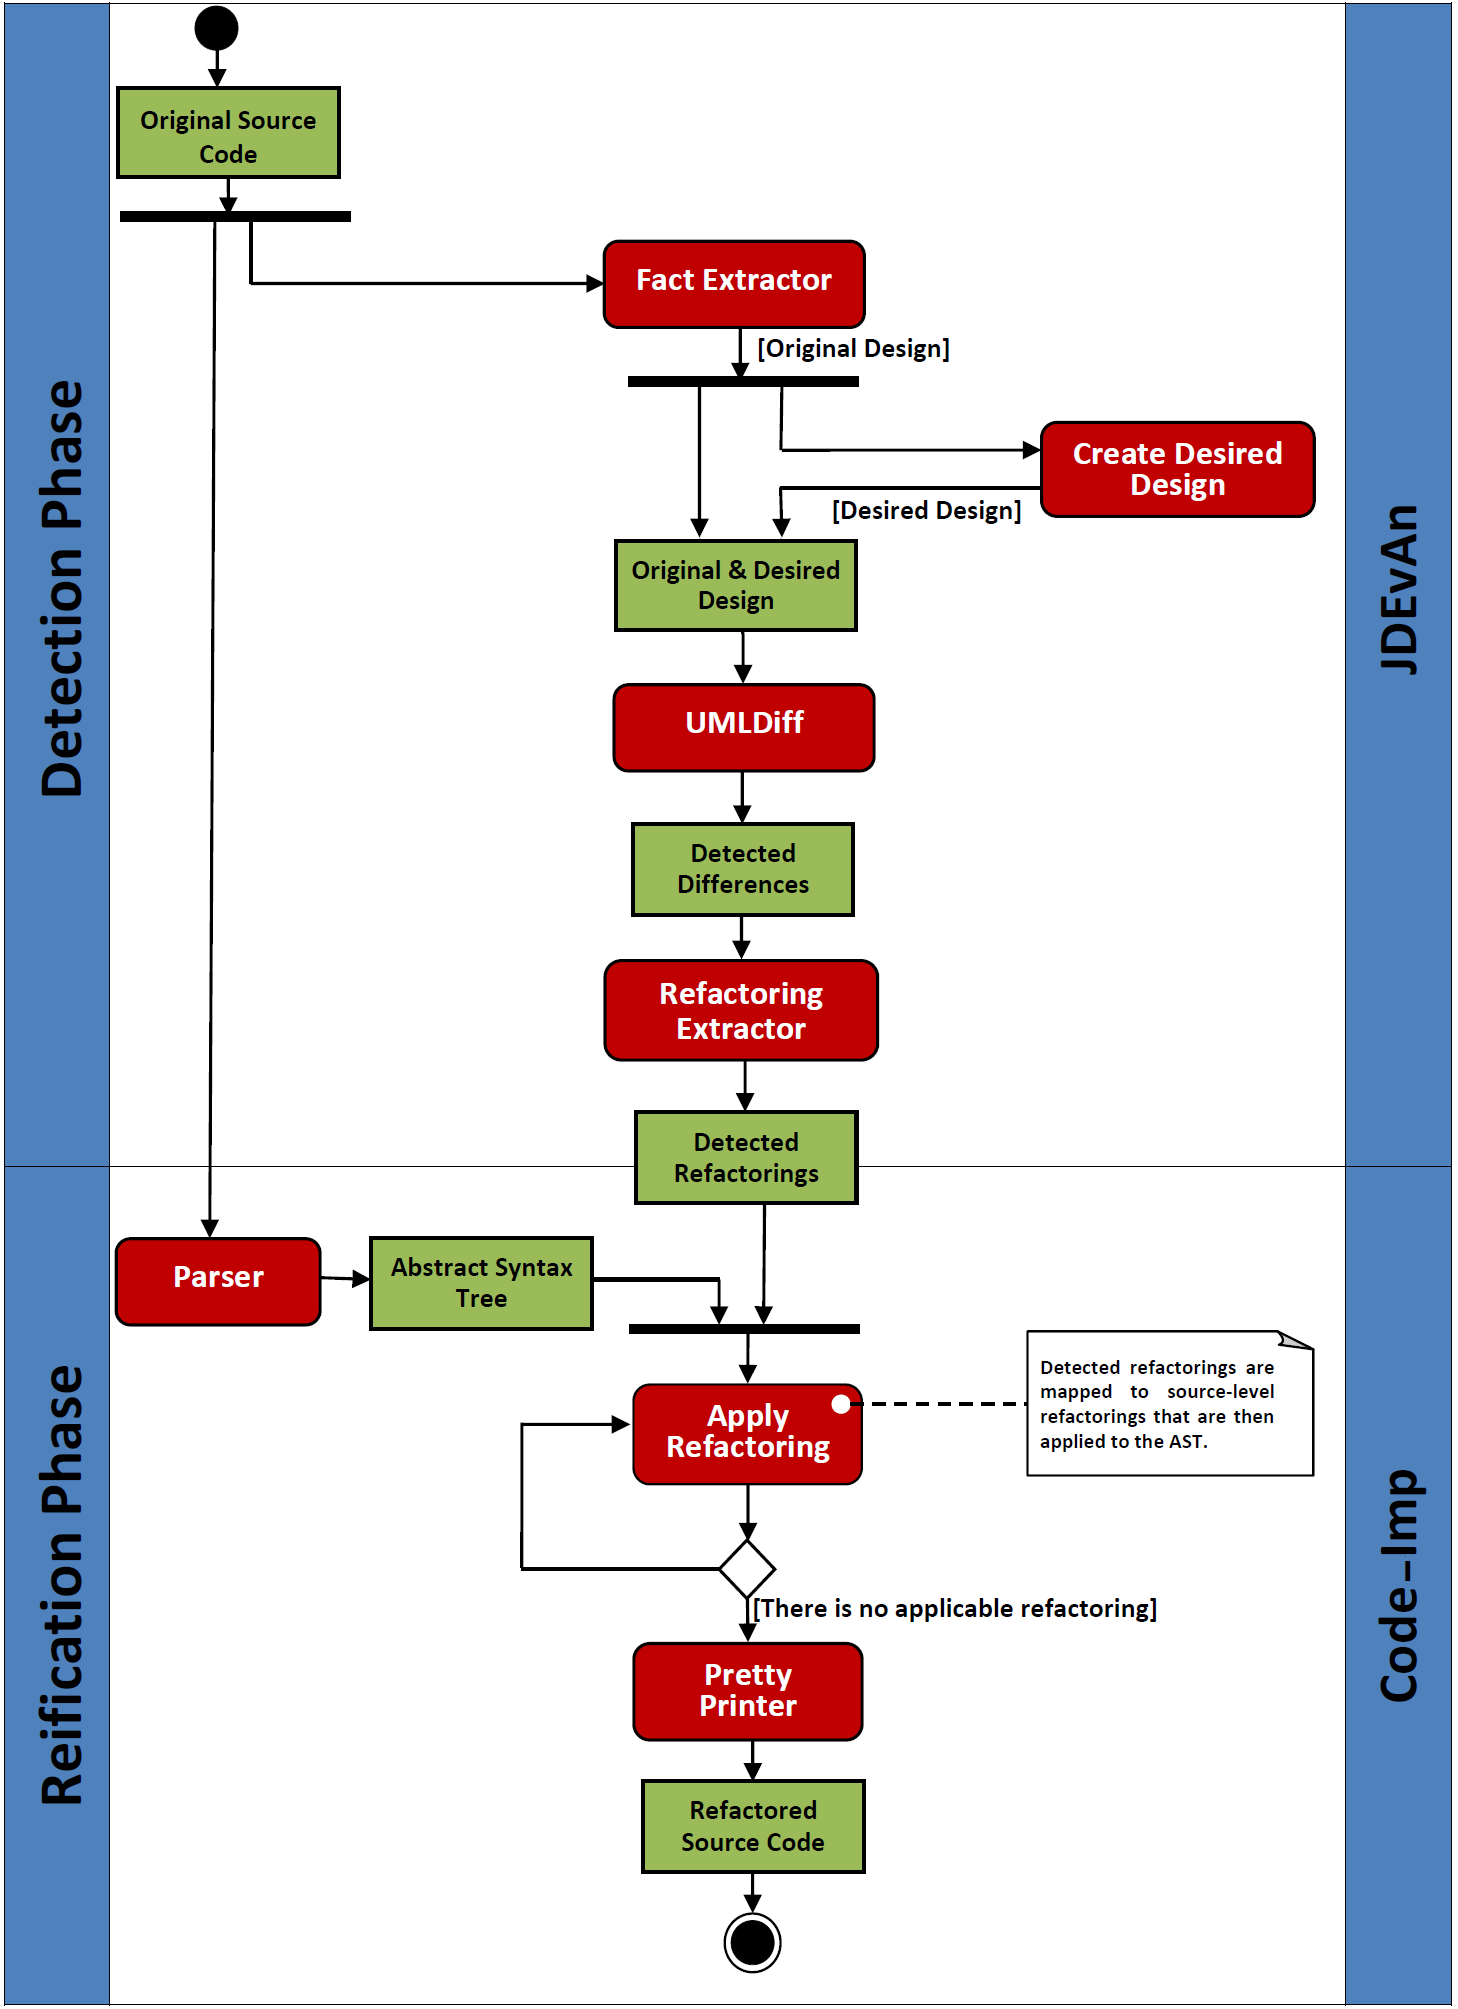
\includegraphics[width=0.8\linewidth]{bilder/designdiff.png}
      \end{figure}
    \end{column}
    \begin{column}{.5\textwidth}
      \begin{itemize}
        \item JDEvAn
        \begin{itemize}
          \item Item
          \item Item
        \end{itemize}
        \item Code-Imp
        \begin{itemize}
          \item Item
          \item Item
        \end{itemize}
      \end{itemize}
    \end{column}
  \end{columns} 
\end{frame}

\subsection{The Spartanizer: Massive Automatic Refactoring}

\begin{frame}{The Spartanizer: Massive Automatic Refactoring}
  \begin{itemize}
    \item Tool demo paper
    \item Eclipse plugin for automatic refactoring to make code more compact
    \pause
    \item Shows that automatic refactoring can be used effectively
  \end{itemize}
\end{frame}

\begin{frame}[fragile]{The Spartanizer: Massive Automatic Refactoring}
  \begin{columns}[T]
    \begin{column}{.49\textwidth}
      \lstinputlisting{code/C0.java}
    \end{column}
    \begin{column}{.5\textwidth}
      \lstinputlisting{code/C1.java}
    \end{column}
  \end{columns}
\end{frame}

\section{Evaluation}

\begin{frame}{Evaluation} 
  \begin{itemize}
    \item Item
    \item Item
  \end{itemize}
\end{frame}

\begin{frame}{Evaluation} 
  \begin{table}[htb]
    \centering
    \caption{Comparison with respect to achieved goals}
    \label{tbl:goals}
    \begin{tabular}{r|ccc}
      ~               & Understandability & Correctness & Maintainability \\ \hline
      C to C++        & +                 & +           & + \\
      Polymorphism    & o                 & +           & + \\
      Design Diff.    & o                 & +           & + \\
      JDEvAn          & o                 & -           & + \\
      Code-Imp        & o                 & -           & + \\
      The Spartanizer & +                 & o           & + \\
    \end{tabular}
  \end{table}
\end{frame}

\begin{frame}{Evaluation}
  \begin{table}[htb]
    \centering
    \caption{Comparison with respect to supported steps}
    \label{tbl:steps}
    \begin{tabular}{r|ccc}
      ~               & Detection & Identification  & Execution \\ \hline
      C to C++        & o         & o               & o \\
      Polymorphism    & o         & o               & - \\
      Design Diff.    & -         & o               & + \\
      JDEvAn          & +         & +               & + \\
      Code-Imp        & +         & +               & + \\
      The Spartanizer & o         & +               & + \\
    \end{tabular}
  \end{table}
\end{frame}

\appendix
\section*{\appendixname}

\begin{frame}{Papers}
  \begin{thebibliography}{10}
    \beamertemplatearticlebibitems
    
    \bibitem{polymorphism}
      Demeyer
      \newblock Maintainability versus Performance: What's the Effect of Introducing Polymorphism?
      \newblock {\em Technical Report, Lab. on Reengineering, Universiteit Antwerpe}, 2002
    
    \bibitem{coevolution}
      D'Hondt, De Volder, Mens, Wuyts
      \newblock Co-evolution of Object-Oriented Software Design and Implementation
      \newblock {\em Software Architectures and Component Technology}, 2002
    
    \bibitem{design-diff}
      Moghadam, Ó Cinnéide
      \newblock Automated Refactoring using Design Differencing
      \newblock {\em 16th European Conference on Software Maintenance and Reengineering (CSMR)}, 2012
  \end{thebibliography}
\end{frame}

\begin{frame}{Papers}
  \begin{thebibliography}{10}
    \beamertemplatearticlebibitems
    
    \bibitem{cpp}
      Fanta, Rajlich
      \newblock Restructuring Legacy C Code into C++
      \newblock {\em IEEE International Conference on Software Maintenance (ICSM)}, 1999
    
    \bibitem{sparta}
      Gil, Orrù
      \newblock The Spartanizer: Massive Automatic Refactoring
      \newblock {\em 24th International Conference on Software Analysis, Evolution and Reengineering (SANER)}, 2017
  \end{thebibliography}
\end{frame}

\end{document}
